%! Author = lili
%! Date = 9/7/26

\section{Genotyping mittels PCR, Arabidopsis CRISPR Mutante}\label{sec:genotyping-mittels-pcr-arabidopsis-crispr-mutante}

\subsection{Einführung}\label{subsec:einfuhrung2}

\defin{sgrna}

\begin{figure}[H]
    \centering
    \begin{subfigure}[t]{0.45\textwidth}
        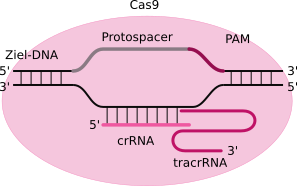
\includegraphics[width=0.8\linewidth]{images/cas9_cr_tracr}
        \caption{Vergleich}\label{fig:cas9_cr_tracr}
    \end{subfigure}
    \hfill
    \begin{subfigure}[t]{0.45\textwidth}
        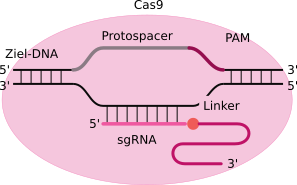
\includegraphics[width=0.8\linewidth]{images/cas9_sg}
        \caption{Vergleich}\label{fig:cas9_sg}
    \end{subfigure}
    \caption{Vergleich}\label{fig:cas9_cr_tracr_cas9_sg}
\end{figure}

%\subsection{DNA Extraktion}



%\subsection{PCR zur Genotypisierung}


%\subsection{Agarosegelelektrophorese}




\kfrage{wurzelbalsgalle}
\kfrage{opineAgrobakterium}
\kfrage{transformationsubstanzen}
\kfrage{bandenmuster}
\frage{genotypphaenotyp}
\frage{vorwaertsrueckwaerts}
\frage{crispr}
\frage{arabidopsismodell}
\frage{kontrollenpcr}
\frage{gelelektrophorese}
\frage{ncoicaps}
